\documentclass[11pt,xcolor=dvipsnames,professionalfonts,notes]{beamer}

% Pakete
\usepackage[utf8]{inputenc}
\usepackage[english]{babel}

% AMS Pakete
\usepackage{amsmath}
\usepackage{amsfonts}
\usepackage{amssymb}

% Einheiten
\usepackage{siunitx}
\sisetup{
	separate-uncertainty
}

% Grafiken
\usepackage{graphicx}
\usepackage{tabularx}
\setbeamerfont{caption}{size=\footnotesize}
\setbeamertemplate{caption}{\raggedright\insertcaption\par}

% Theme
\usetheme{Boadilla}
\usecolortheme{rose}
\useoutertheme{infolines}
\useinnertheme{rectangles}
\setbeamertemplate{itemize subitem}[triangle]

\usefonttheme[onlymath]{serif}

% [num] Zitationen
\setbeamertemplate{bibliography item}[text]

% Navigationsleiste ausschalten
\beamertemplatenavigationsymbolsempty

\author[Christopher Deutsch]
{Christopher Deutsch}

\title
{Interactions of photons with matter}

\subtitle
{}
%\logo{}

\institute[]
{Joint BCGS Seminar on Detectors in Nuclear and Particle Physics\\ Summer Term 16}

\date{2.\ May 2016}

%\setbeamercovered{transparent}
%\setbeamertemplate{navigation symbols}{}

\newcommand{\beginbackup}{
	\newcounter{framenumbervorappendix}
	\setcounter{framenumbervorappendix}{\value{framenumber}}
}
\newcommand{\backupend}{
	\addtocounter{framenumbervorappendix}{-\value{framenumber}}
	\addtocounter{framenumber}{\value{framenumbervorappendix}} 
}

\begin{document}
\maketitle

\begin{frame}{Interactions of photons with matter}
	\tableofcontents
\end{frame}

\note[itemize]{
	\item Photoelectric effect
	
	\item Compton effect
	
	\item Pair production
	
	\item Electromagnetic showers
	
	\item Detector concepts		
}

\section{Introduction}

\subsection{Charged particle interaction}

\begin{frame}{Introduction -- charged particle interactions}
	Interaction of \textbf{charged particles} with matter:
	\begin{itemize}
		\item energy loss due to inelastic collisions with atomic electrons
		\item range $R$
	\end{itemize}
	\vfill
	\begin{center}
		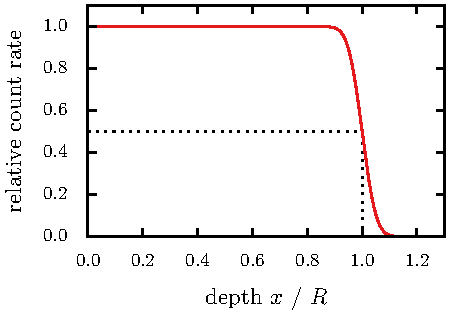
\includegraphics{./figures/range.pdf}
	\end{center}
\end{frame}

\note[itemize]{
	\item charged particles
	\begin{itemize}
		\item fixed range
	\end{itemize}
	
	\item photons
	\begin{itemize}
		\item uncharged
	\end{itemize}
}


\subsection{Photon interaction}

\begin{frame}{Introduction -- photon interactions}
	\begin{columns}
		\column[c]{0.4\textwidth}
			\begin{center}
				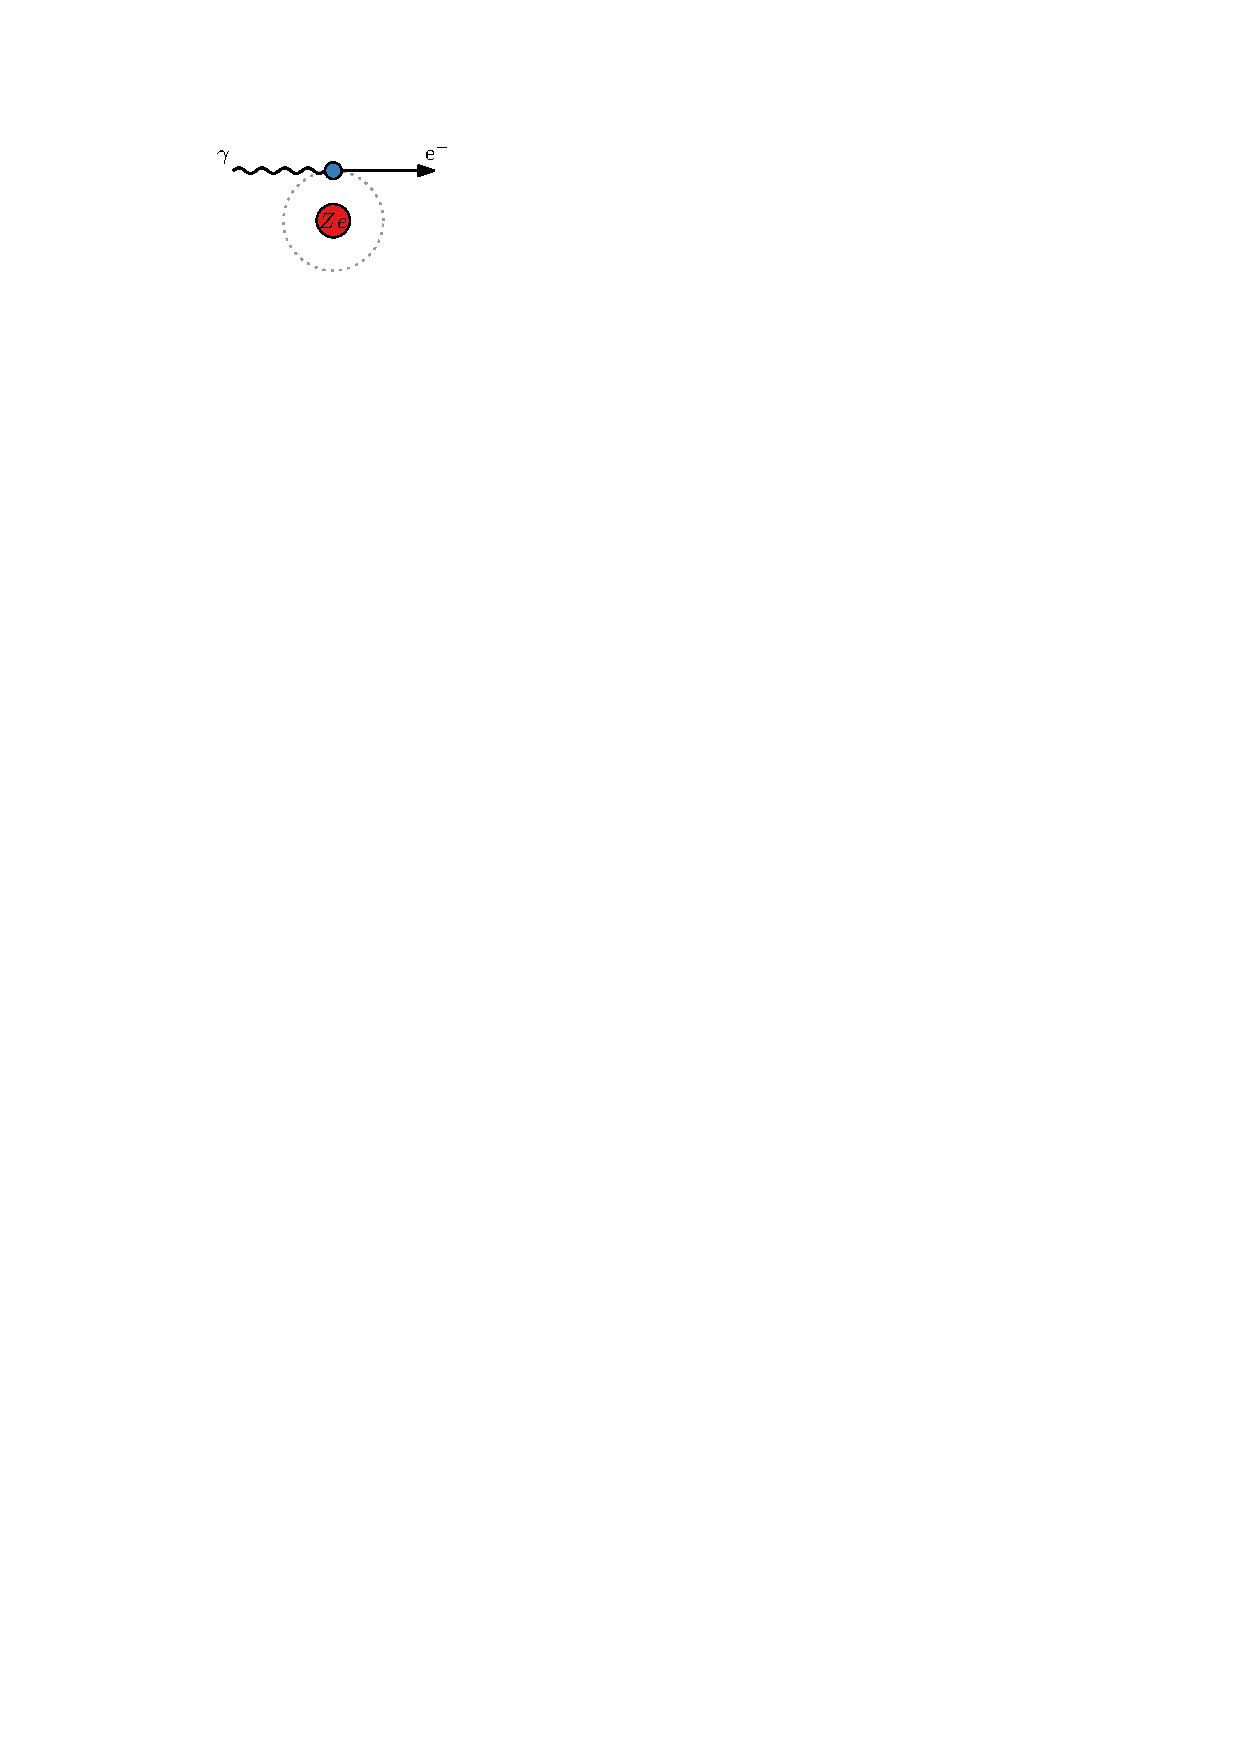
\includegraphics{./figures/photoeffect_intro.pdf}
			\end{center}
		
		\column[c]{0.6\textwidth}
			Photoelectric effect
	\end{columns}
	\vspace{-0.2cm}
	\begin{columns}
		\column[c]{0.4\textwidth}
		\begin{center}
			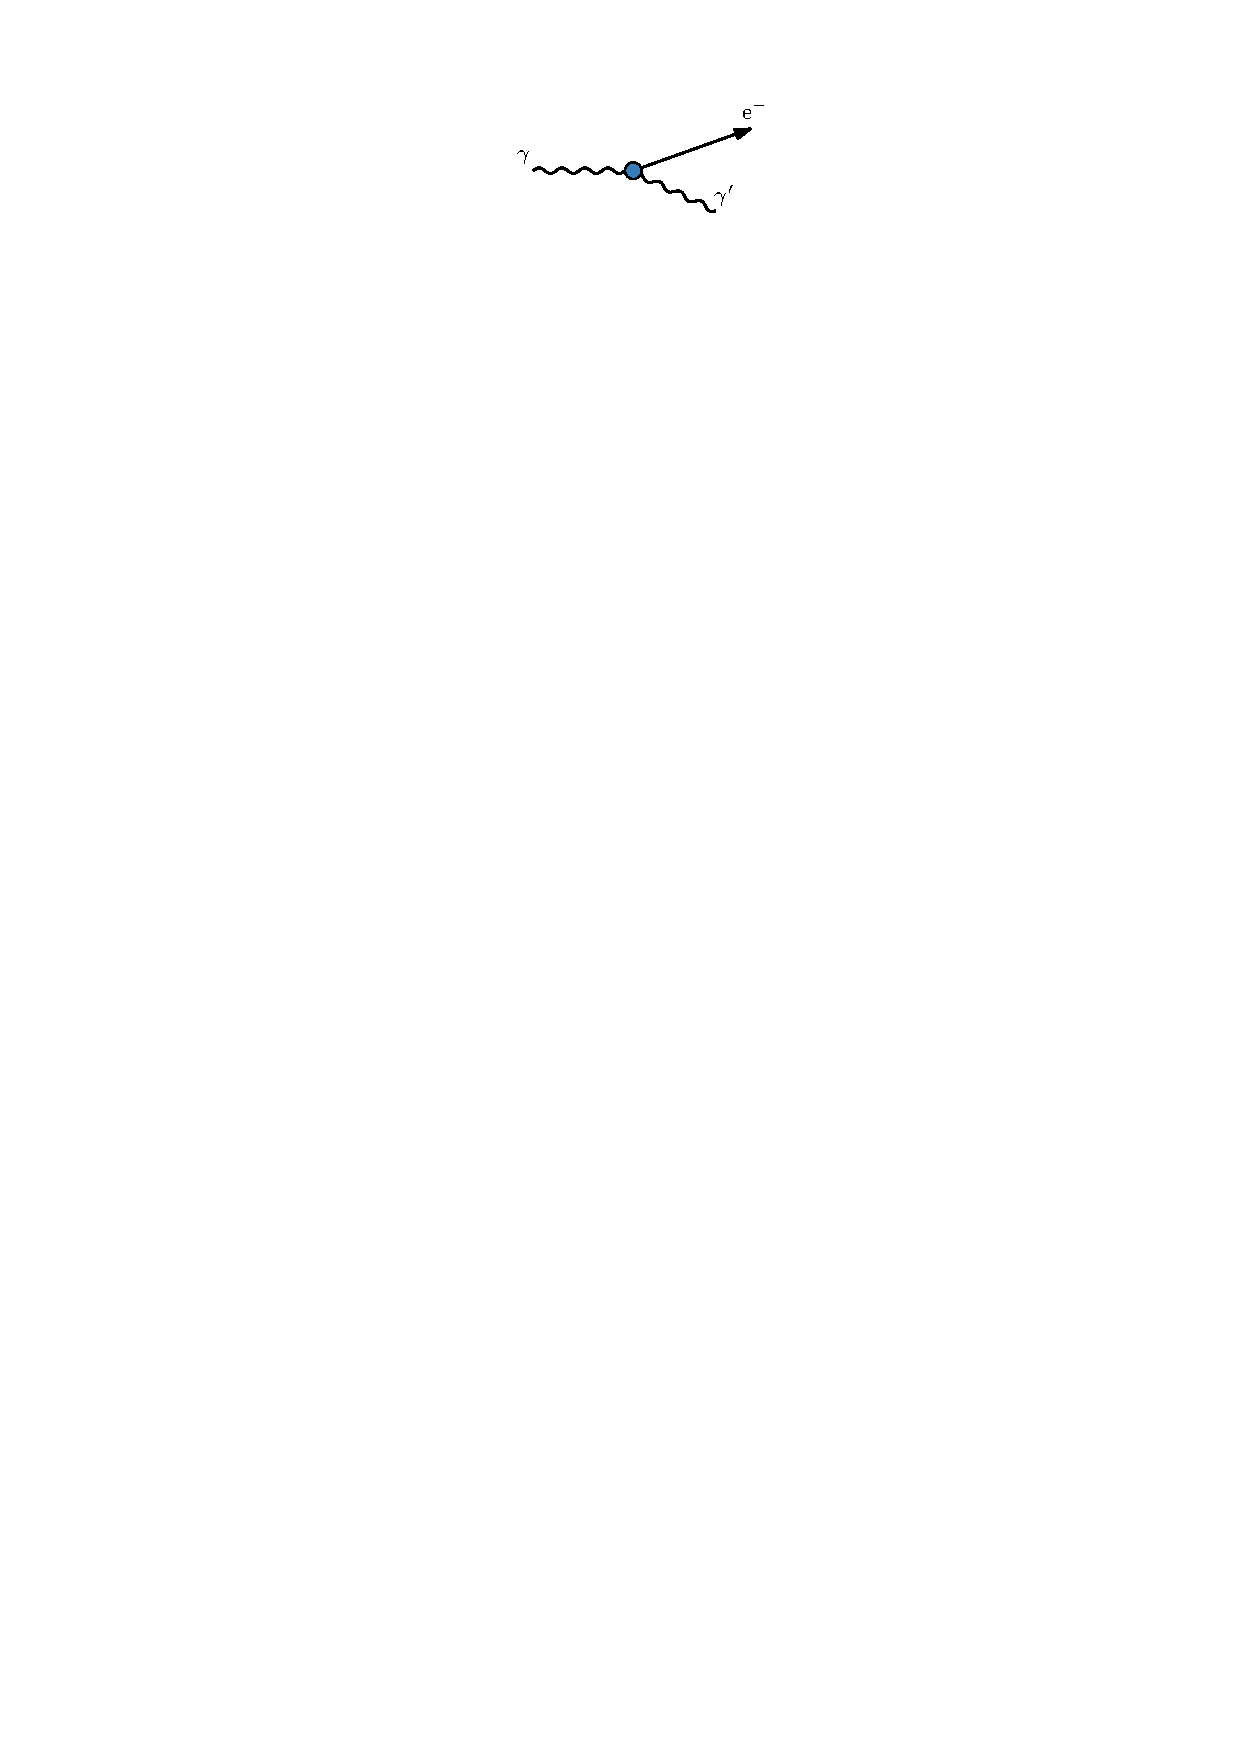
\includegraphics{./figures/compton_intro.pdf}
		\end{center}
		
		\column[c]{0.6\textwidth}
		Compton effect
	\end{columns}
	\vspace{0.2cm}
	\begin{columns}
		\column[c]{0.4\textwidth}
		\begin{center}
			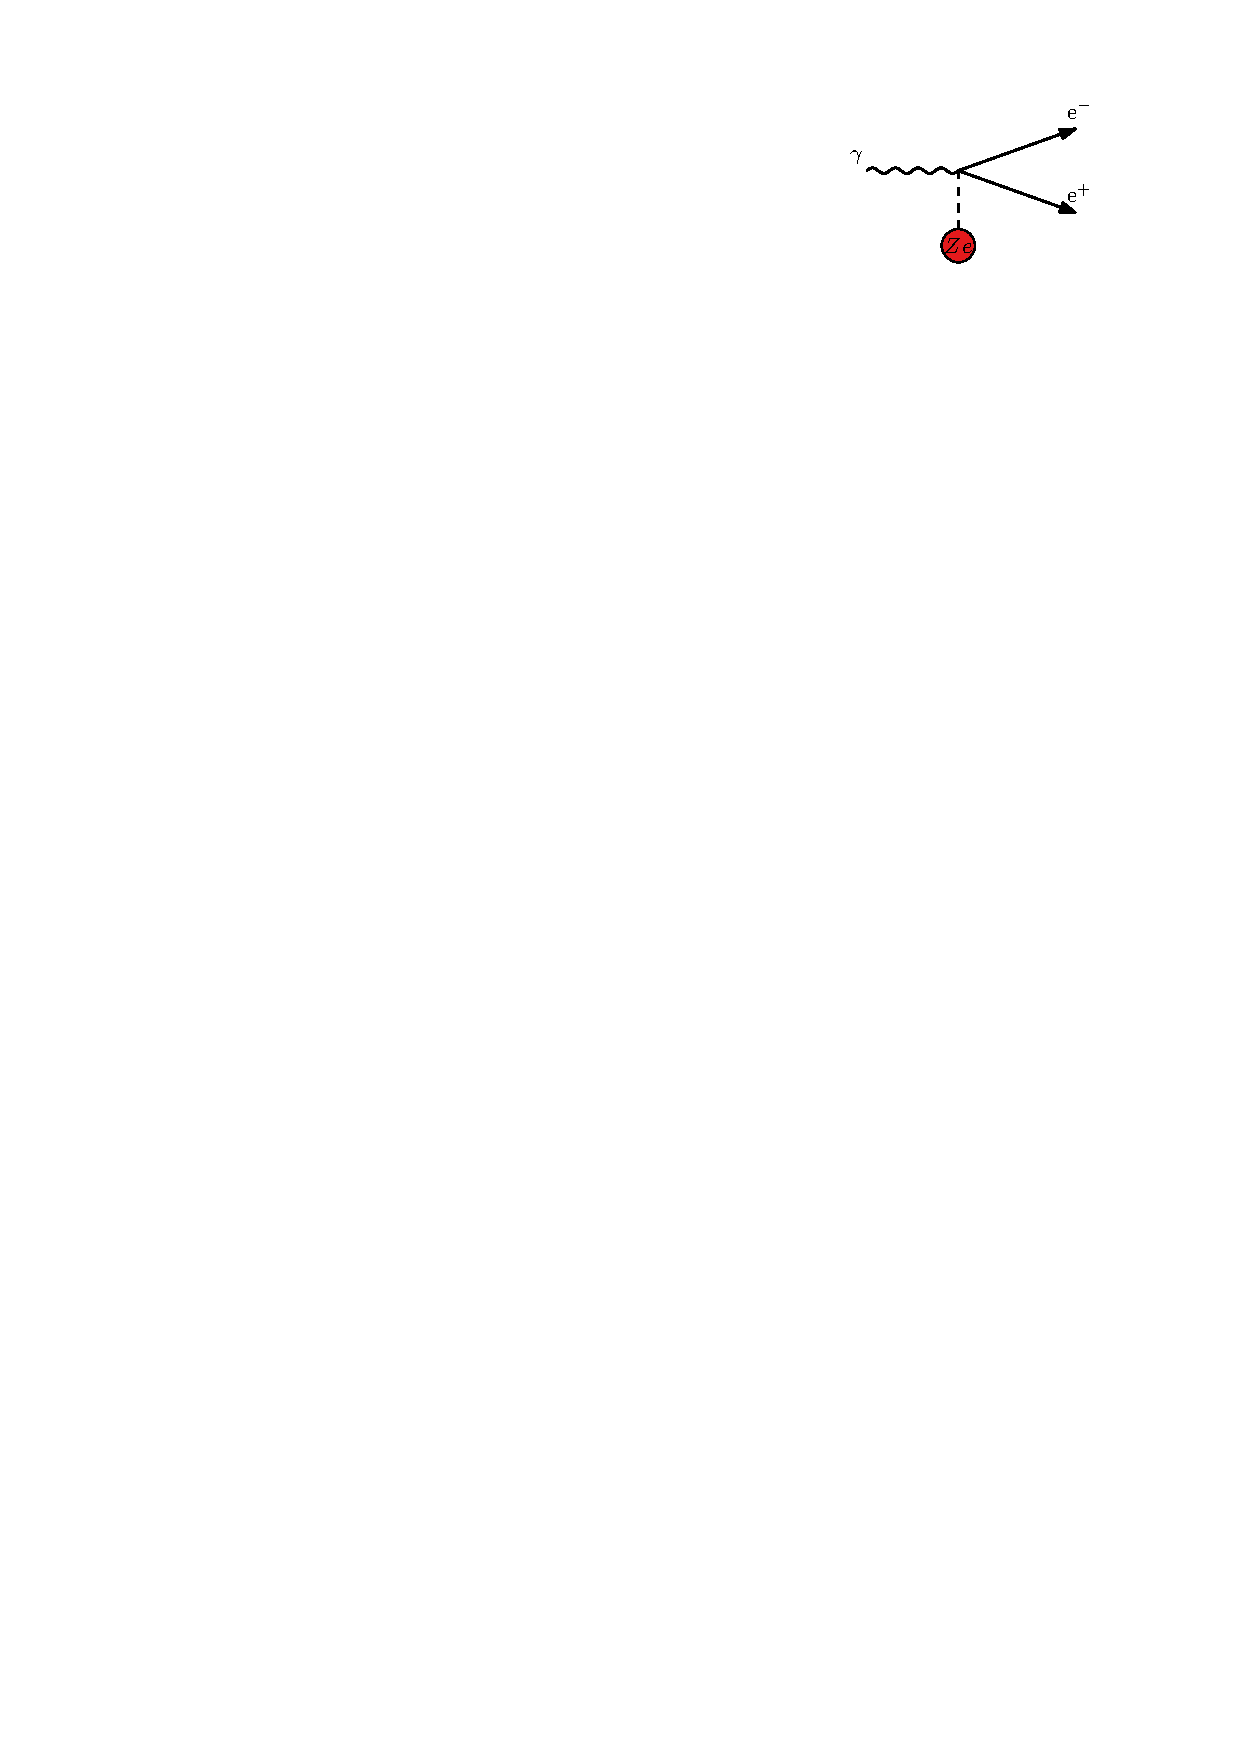
\includegraphics{./figures/pair_intro.pdf}
		\end{center}
		
		\column[c]{0.6\textwidth}
		Pair production
	\end{columns}
\end{frame}

\note[itemize]{
	\item (independent) proccesses relevant in energy range (\si{keV} -- \si{GeV}) for nuclear \& detector physics
	
	\item photoelectric effect:
	\begin{itemize}
		\item photon absorbed by atomic electron
		\item electron liberated
		\item dominant at low energies
	\end{itemize}
	
	\item compton scattering:
	\begin{itemize}
		\item scattering of photons at free / quasifree electrons
		\item dominant at intermediate energies
	\end{itemize}
	
	\item pair production:
	\begin{itemize}
		\item $\mathrm{e}^+ \mathrm{e}^-$ production in Coulomb field
		\item dominant at high energies
	\end{itemize}
	
	\item other processes:
	\begin{itemize}
		\item Thomson \& Rayleigh scattering (?)
	\end{itemize}
}

\begin{frame}{Introduction -- Lambert-Beer law}
	\begin{columns}
		\column[t]{0.6\textwidth}
		Photon beam passing through matter:
			\begin{itemize}
				\item interaction removes $\gamma$ from beam by absorption or scattering
				\begin{itemize}
					\item individual $\gamma$ do not lose energy
					\item beam intensity is attenuated
				\end{itemize}
				
				\item attenuation:
				\begin{align*}
					\mathrm{d} I = - \mu I \mathrm{d}x
				\end{align*}
				\begin{itemize}
					\item Lambert-Beer law:
					\begin{align*}
					I(x) = I_0 \, e^{-\mu x}
					\end{align*}
				\end{itemize}
				
				
				\item mean free path
				\begin{align*}
					\lambda = \frac{1}{\mu}
				\end{align*}
			\end{itemize}

		\column[t]{0.4\textwidth}		
			\begin{center}
				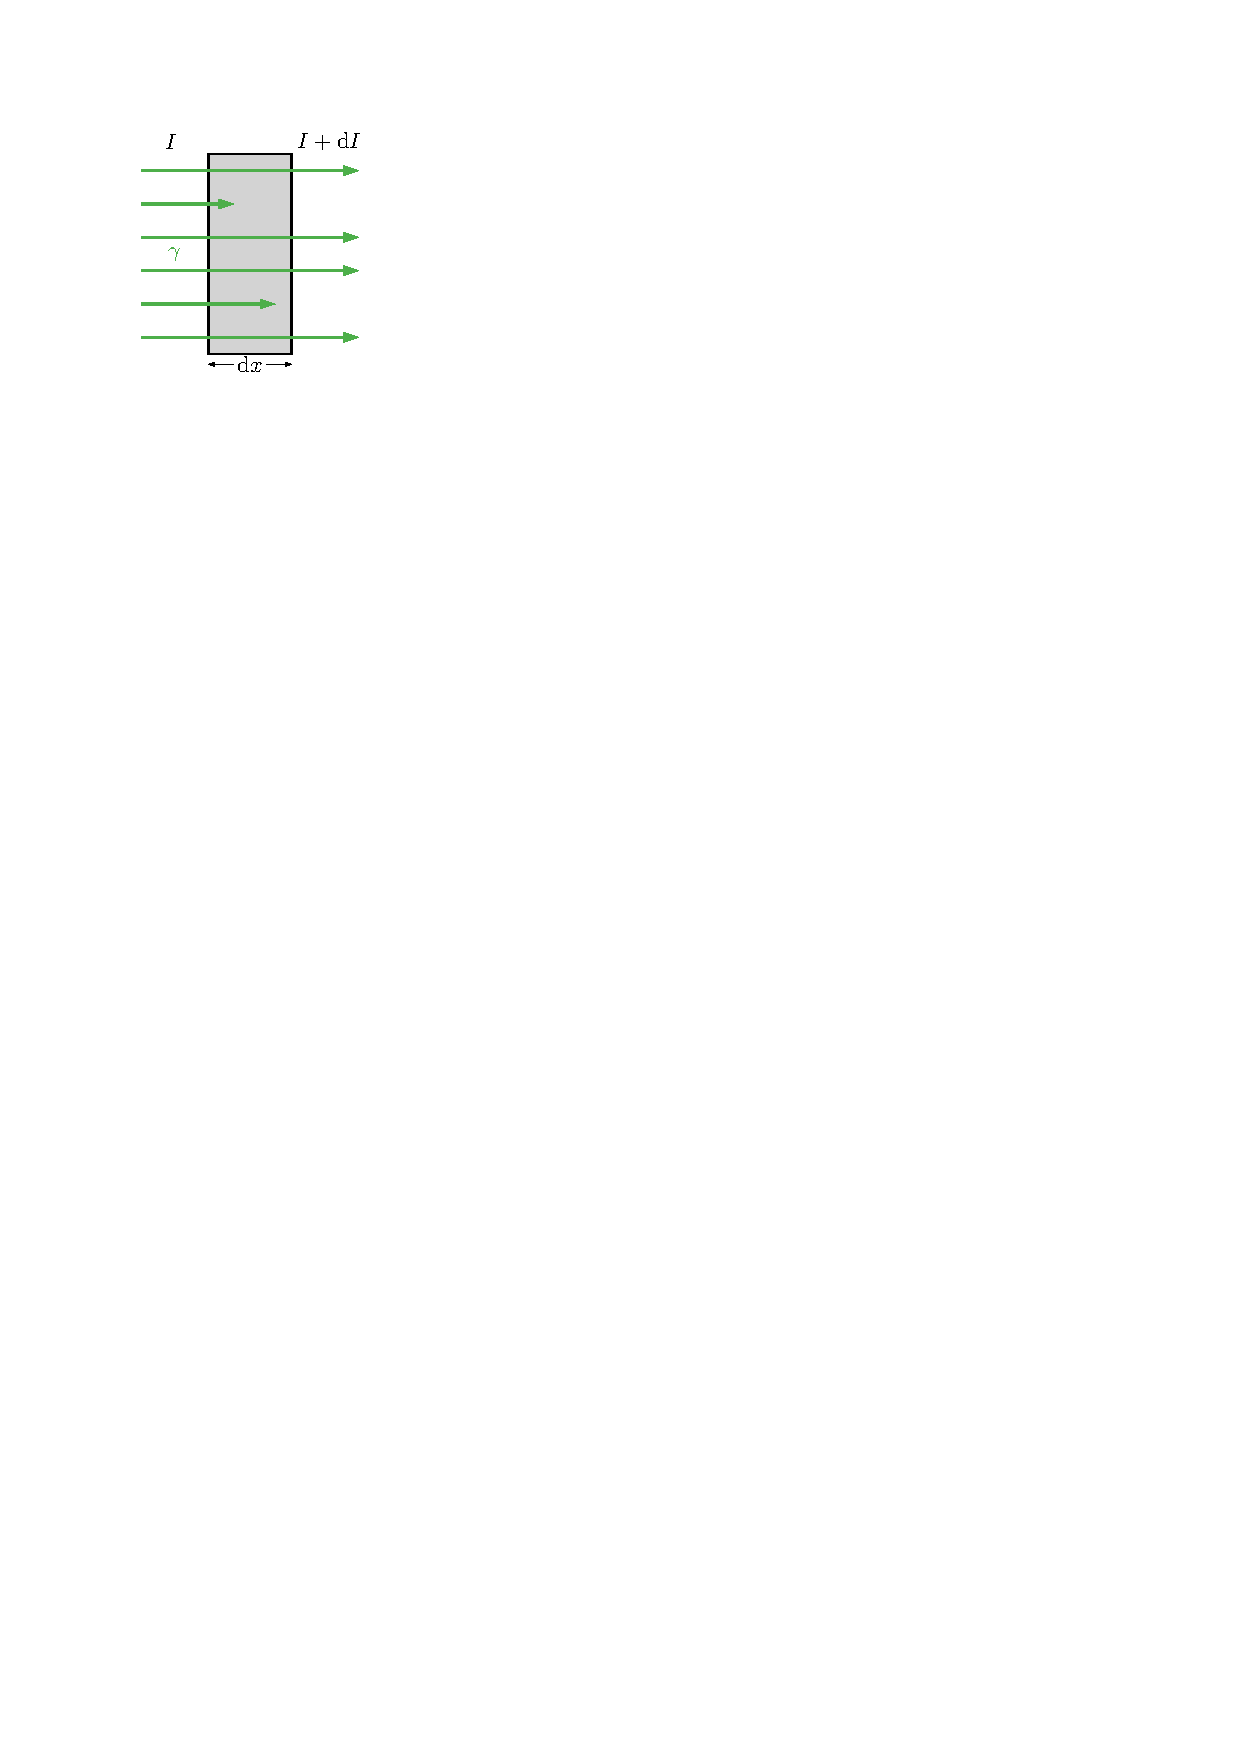
\includegraphics{./figures/lambert_beer.pdf}
			\end{center}			
	\end{columns}
\end{frame}

\note[itemize]{
	\item absorption coefficient material and energy dependent 
}

\begin{frame}{Introduction -- range comparison}
	
	\begin{columns}
		\column[t]{0.5\textwidth}
		\centering
		\hspace{1cm}\textbf{charged particles:}
		
		\vspace{0.5cm}
		
		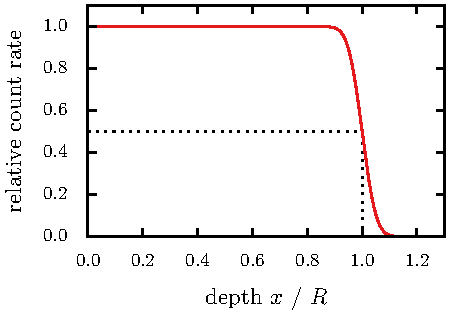
\includegraphics[width=1.0\textwidth]{./figures/range.pdf}
		
		\column[t]{0.5\textwidth}
		\centering
		\hspace{1cm}\textbf{photons:}
		
		\vspace{0.5cm}
		
		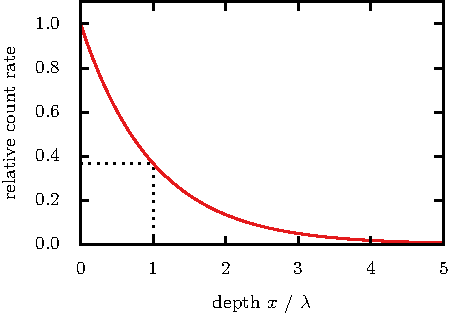
\includegraphics[width=1.0\textwidth]{./figures/lambert_beer_exp.pdf}
		
	\end{columns}
\end{frame}

\note[itemize]{
	\item charged particles gradually lose energy until stop at a fixed range
	\item photons don't lose energy but are absorbed or scattered from the beam	
}


\begin{frame}{Introduction - absorption coefficient}
	\begin{itemize}
		\setlength\itemsep{2.em}
		\item absorption coefficient
		\begin{align*}
			\mu = n \sigma
		\end{align*}
		$n$: density of atoms \\
		$\sigma$: total absorption/scattering cross section per atom
		
		\item cross section per atom
		\begin{align*}
			\sigma = \sigma_\mathrm{photo} + Z \cdot \sigma_\mathrm{Compton} + \sigma_\mathrm{pair}
		\end{align*}
		\begin{itemize}
			\item depends on material \& photon energy
		\end{itemize}
		
		
		
		

		
	\end{itemize}	
\end{frame}

\note[itemize]{
	\item neglect other processes ($Z$?) (processes independent)
	
	\item higher penetration power
	\begin{itemize}
		\item smaller cross section cmp.\ inelastic $\mathrm{e}^-$ collision
	\end{itemize} 
}

\section{Interaction processes}

\begin{frame}{Interaction processes}
	\centering
	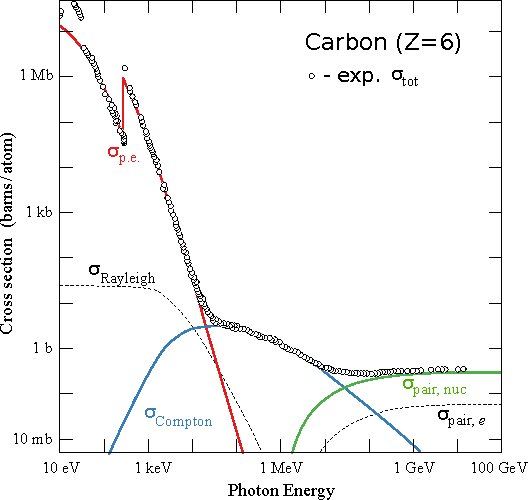
\includegraphics[scale=0.9]{./figures/carbon.pdf}
\end{frame}
\begin{frame}{Interaction processes}
	\centering
	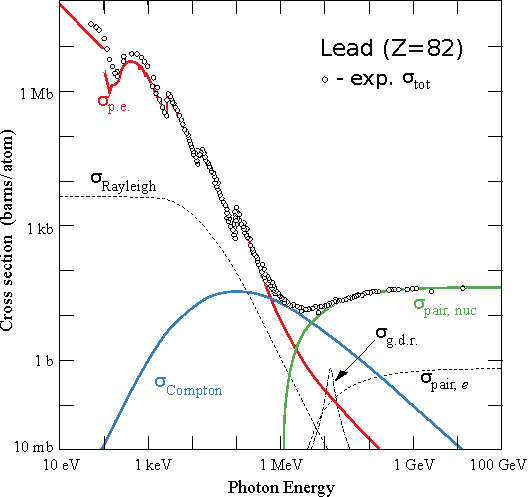
\includegraphics[scale=0.9]{./figures/lead.pdf}
\end{frame}

\begin{frame}{Interaction processes}
	dominant interactions at photon energies $E_\gamma$?\\
	dominant interactions for atomic number $Z$?
	\begin{itemize}
		\item photoelectric effect: $E_\gamma < \SI{1}{MeV}$
		\item Compton scattering: $E_\gamma \approx \SI{1}{MeV}$
		\item pair production: $E_\gamma > \SI{1}{MeV}$
	\end{itemize}
\end{frame}

\subsection{Photoelectric effect}

\begin{frame}{Photoelectric effect}
	\begin{itemize}
		\item absorption of photon by atomic electron (illustration) (free electron -- forbidden: recoil momentum)
		\item $E = h \nu - E_\mathrm{b}$
		\item complete transfer of energy
		\item cross section -- shell structure
		\begin{itemize}
			\item absorption-edges
			\item K-shell dominant for high energies
		\end{itemize}
		nonrelativistic but $E_\gamma > E_\mathrm{b, K}$:
		\begin{align*}
			\sigma_\mathrm{photo} = \frac{32 \pi}{3} \sqrt{2} r_\mathrm{e}^2  \alpha^4  Z^5 \left( \frac{m_\mathrm{e} c^2}{E_\gamma}\right)^\frac{7}{2} 
		\end{align*}		
	\end{itemize}
\end{frame}

\begin{frame}{Sketch}

\end{frame}


\subsection{Compton scattering}

\begin{frame}{Compton scattering}
	\begin{itemize}
		\item
	\end{itemize}
\end{frame}

\subsection{Pair production}

\begin{frame}{Pair production}
	\begin{itemize}
		\item
	\end{itemize}
\end{frame}



\section{Electromagnetic showers}

\section{Detector concepts}

\begin{frame}{Detector concepts}
	\begin{itemize}
		\item PMT
	\end{itemize}
\end{frame}


\begin{frame}{Bibliography}
	\begin{thebibliography}{1000}
		\bibitem[Leo]{leo}
			W.\ R.\ Leo,
			\emph{Techniques for Nuclear and Particle Physics Experiments},
			Springer (1994).
		
		\bibitem[Sieg]{siegbahn}
			C.\ M.\ Davisson,
			\emph{Interaction of $\gamma$-Radiation with Matter},
			published in K.\ Siegbahn (ed.),
			\emph{Alpha- Beta- and Gamma-Ray Spectroscopy}, North-Holland Publishing Company (1979).
		
		\bibitem[PDG]{pdg}
	\end{thebibliography}
\end{frame}

\beginbackup

\begin{frame}{Appendix}
\end{frame}

\backupend

\end{document}